\subsection{Pattern Matching DTW}
\newcommand{\dd}{\mathinner{..}}

\begin{frame}
  \centering
  {\Large Pattern Matching Under Dynamic Time Warping Distance}

  \bigskip
  {\large SPIRE'22}\\
  \bigskip
  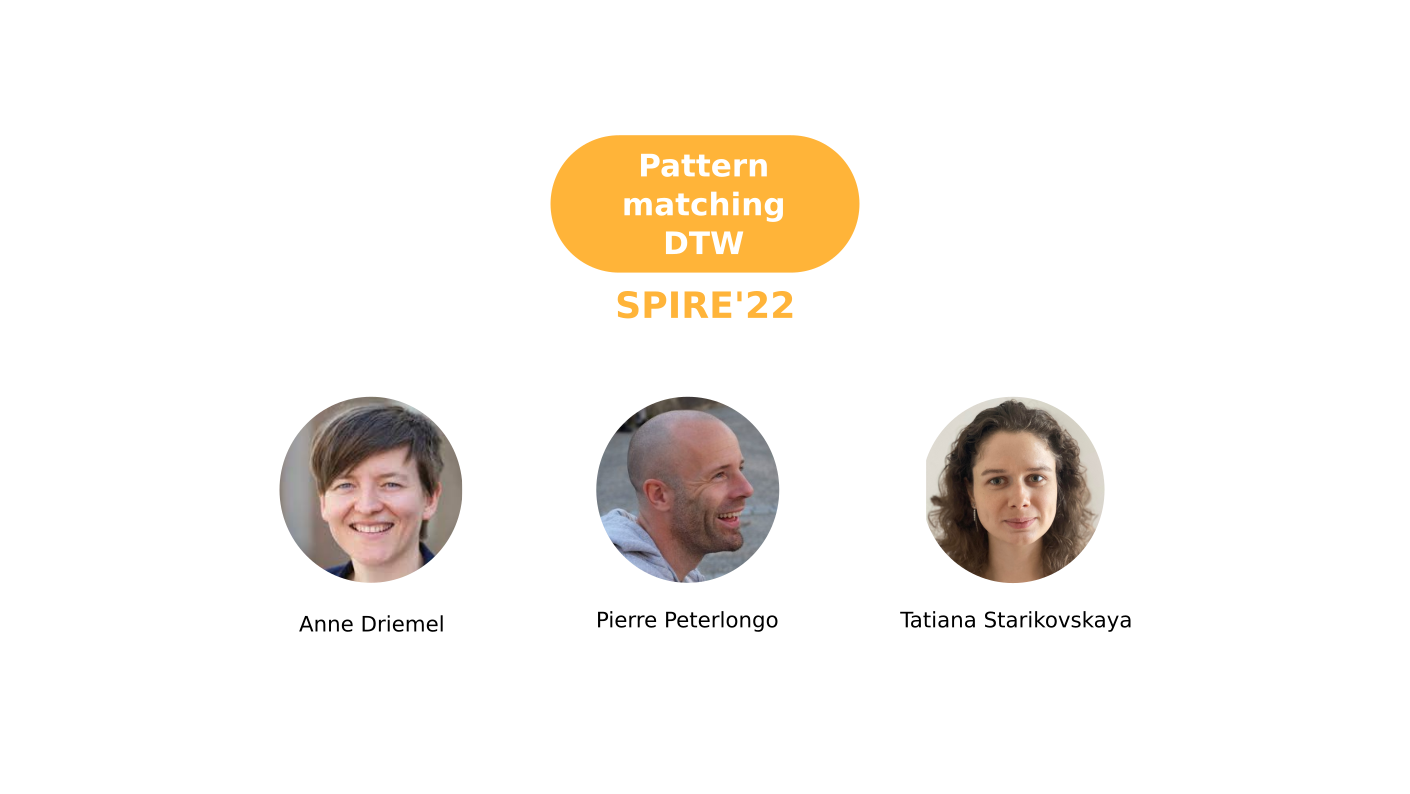
\includegraphics{pictures/mindmap/dtw.png}

  \bigskip
  Anne Driemel, Pierre Peterlongo, Tatiana Starikovskaya
\end{frame}

\begin{frame}{Formal definition of $\dtw(X,Y)$ and dynamic programming}

  \begin{columns}
  \column{0.45\textwidth}
  \newcommand{\dtwgrid}[2]{% height width 
\foreach \i in {0,...,#1} {
	\foreach \j in {0,...,#2} {
		\filldraw[black] (\i , \j) circle (2pt);
		\ifthenelse{ \not \equal{#2}{\j}}{ 
			\draw[->] ($(\i , \j+0.9)$) -- ($(\i , \j+0.1)$);
		}{}
		\ifthenelse{ \not \equal{#1}{\i}}{
  			\draw[->] ($(\i +0.1 , \j)$) -- ($(\i +0.9 , \j)$);
		}{}
		\ifthenelse{\not\equal{#1}{\i} \and \not \equal{#2}{\j}}{%
  			\draw[->] ($(\i +0.1 , \j + 0.9)$) -- ($(\i +0.9, \j + 0.1)$);
  		}{}
	}
}
}

\newcommand{\dtwarrow}[2]{%
\draw[->,line width=0.3mm,red] #1 -- #2;
}

  \begin{figure}
      \beamermathcolor{black}
      \centering
      \begin{tikzpicture}[scale=0.8, every node/.style={scale=1.2}]
      \dtwgrid{5}{2}
  
      \foreach \i in {1,...,6} {
          \node at ($(\i-1, 2.8)$) {\tiny{$X[\i]$}};
      }
      \foreach \j in {1,...,3} {
          \node at ($(-1.2, 3 -\j )$) {\tiny{$Y[\j]$}};
      }
  
      \foreach \x[count=\i] in {C,A,A,A,G,G} {
          \node at ($(\i-1 , 2.3)$) {\textcolor{black}{\tiny{\x}}};
      }
      \foreach \y[count=\j] in {A,T,G} {
          \node at ($(-0.5, 3 -\j )$) {\textcolor{black}{\tiny{\y}}};
      }
  
  
      \only<2->{
          \dtwarrow{(0.1,2)}{(0.9,2)}
          \dtwarrow{(3.1,1.9)}{(3.9,1.1)}
          \dtwarrow{(1.1,2)}{(1.9,2)}
          \dtwarrow{(2.1,2)}{(2.9,2)}
          \dtwarrow{(4,0.9)}{(4,0.1)}
          \dtwarrow{(4.1,0)}{(4.9,0)}
          \node at (5,-0.3) {\bred{$\pi$}};
      }
  
      \end{tikzpicture}
  \end{figure}
  \column{0.45\textwidth}
  \centering
  \only<3>{
  $\text{cost}(\pi) = \sum_{(i,\ j)\in \pi} d(X[i],Y[j])$\\
  \vspace{0.5cm}
  $\dtw(X,Y) = \min_{\pi} \text{cost}(\pi)$\\
  \vspace{0.5cm}
  {\small s.t. $\pi$ goes from top left to bottom right.}}
  \end{columns}
  \pause %grid definition 
  \pause %draw the path
  \pause
  
  \bigskip
  
  
  \only<4|handout:0>{
  \begin{exampleblock}{Path correspondance to alignment}
  \center
  \begin{figure}
  %\missingfigure{Under construction...}
  \centering
  \begin{tikzpicture}[scale=0.7, every node/.style={scale=1}]
  \foreach \x[count=\i] in {C,A,A,A,G,G} {
      \node at ($(\i, 1)$) {\small{\x}};
  }
  \foreach \y[count=\j] in {A,T,G} {
      \node at ($(0.5+\j*1.5, 0)$) {\small{\y}};
  }
  % align A
  \fill[myblue!25] (2, 0.25) -- (2,0.75) -- (4,0.75) -- (2.1,0.25) -- cycle;
  % align G
  \fill[myblue!25] (5, 0.25) -- (5,0.75) -- (6,0.75) -- (5.1,0.25) -- cycle;
  %draw misalignment
  \draw[dashed,red] (1.75, 0.25) -- (1,0.75);
  \draw[dashed,red] (3.5, 0.25) -- (5,0.75);
  \end{tikzpicture}
  \end{figure}
  \vfill
  $\dtw($CAAAG$,$ATG$)=2$
  \end{exampleblock}}
  
  \only<5->{
  
  \btheme{Dynamic Programming solution}\\
  \smallskip
  $D$ a matrix of size $(M+1)(N+1)$ such that $D[i,j]=\dtw(X[1..i],Y[1..j])$\pause
  \bigskip
  
  \btheme{Initialization}~~~$D[0,0]= 0$ and for all $(i,j)$, $D[0,j]=D[i,0]=+\infty$.\\
  \pause
  \bigskip
  \btheme{Recurrence} ~~~ 
      $D[i,j] = \min\{$\beamermathcolor{black}
          $\underbrace{\mathcolor{black!30!blue}{D[i-1,j-1]}}_\text{top-left},
          \underbrace{\mathcolor{black!30!blue}{D[i-1,j]}}_\text{top},
          \underbrace{\mathcolor{black!30!blue}{D[i,j-1]}}_\text{left}$
      $\mathcolor{black!30!blue}{\}+ d(X[i], Y[j])}$.
  }
  
\end{frame}
  

\begin{frame}{}

  \textbf{Our contributions:}\\
  For $T$ and $P$ two strings, $|T|=N$ and  $|P|=M$, $|\RLE(T)|=n$ and  $|\RLE(P)|=m$.
  Pattern matching under DTW distance:
  \begin{itemize}
  \item $\Oh(Nm+nM)$-time general algorithm which can for an integer distance, compute all values bellow $k$ in $\Oh(nmk)$-time. \pause
  \item Toy implementation available on github.\pause
  \item An $\Oh(L^{\eps})$-approximation, for any $0 < \eps < 1$, in  $\Oh(L^{1-\eps} \cdot mn \log^3 L)$-time with $L=\max(N,M)$.\pause
  \item (A $\Oh(n+m)$-time algorithm for $k=1$.)\pause
  \end{itemize}
  
  
  \textbf{Open questions:}
  \begin{itemize}
  \item Is a $\Oh(k(n+m))$-time algorithm possible? \pause
  \item Can those improvements benefit applications?\pause
  \end{itemize}
  \end{frame}


  \begin{frame}{State of the art for DTW on strings}
    $X$ and $Y$ strings, $N=|X|$ and $M=|Y|$.
    \only<3->{With $n$ and $m$ runs in $X$ and $Y$.}\\
    \smallskip
    The dynamic programming takes $\Oh(NM)$ time $=\Oh(N^2)$ in the case $N=M$.\\ \pause
    \begin{block}{No strongly subquadratic [Gold and Sharir]}
    %There are no strongly subquadratic algorithms to compute the DTW distance between two strings over a ternary alphabet unless the Strong Exponential Hypothesis (SETH) is false.
    $|\Sigma| \geq 3 \Rightarrow $ no $\Oh(N^{a})$ time algorithm with $a<2$ unless SETH is false.
    \end{block}\pause

    \ntheme{Run-length compressed} \\
    $\dtw(X,Y)$ can be computed $\Oh(mN+Mn)$-time [Froese et al.] 
    
    \smallskip
    \ntheme{Low distance regime}\\
    If $\dtw(X,Y) \leq k$ it can be computed in $\Oh(kN)$-time [Kuszmaul]
    
    \medskip

    \textcolor{red}{Can we also use (and combine) those approaches for Pattern Matching ?}

\end{frame}

\begin{frame}{Experiments: visualization on simulated data}
  Problem: How to design a protocol that isn't biased towards ED ?\\
  Model to illustrate the impact of homopolymers on ED.
  \begin{center}
    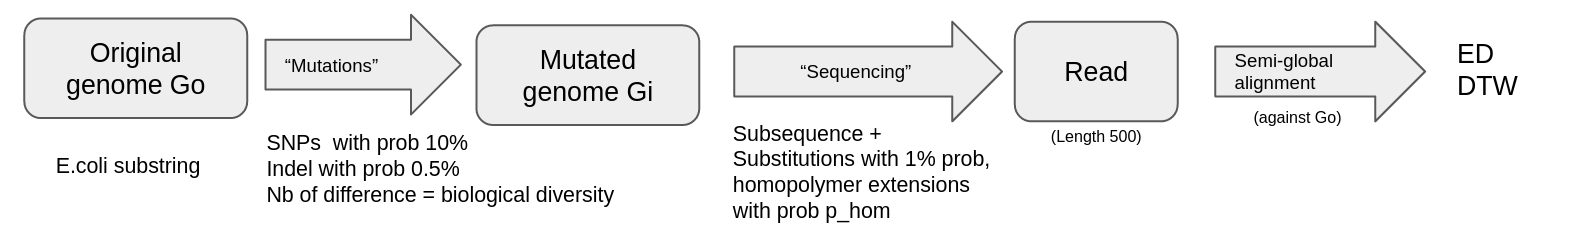
\includegraphics[scale=0.2]{figures/pipeline.png}
  \end{center}
  \vspace{-0.5cm}
  \begin{columns}
    \column{0.3\textwidth}
    
    We compare the values of the two distances as the probability of extending homopolymers increases.
    
    \column{0.5\textwidth}
    \begin{center}
      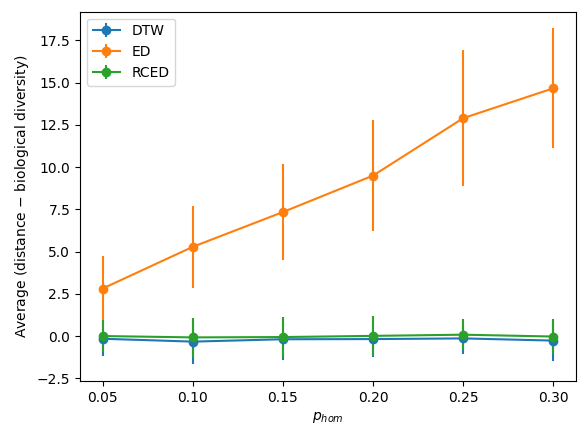
\includegraphics[scale=0.4]{figures/ecoli_10kb_N_100_fixed_ID_0.0005.png}
    \end{center}
  \end{columns}
\end{frame}


\begin{frame}{Comparison to the edit distance}
  \beamermathcolor{black}
  \[
  D[i,j] = {\min\{
  \underbrace{D[i-1,j-1]}_\text{top-left},
  \underbrace{D[i-1,j]}_\text{top},
  \underbrace{D[i,j-1]}_\text{left}
  \} \mathcolor{red}{+ d(X[i], Y[j])}
  }
      \]
  
  \[
  ED[i,j] = {\min\{
  \underbrace{ED[i-1,j-1]}_\text{top-left} \mathcolor{red}{+ d(X[i], Y[j])},
  \underbrace{ED[i-1,j]}_\text{top} \mathcolor{red}{+1},
  \underbrace{ED[i,j-1]}_\text{left} \mathcolor{red}{+1}
  \}
  }
      \]
  
  \pause
  
  \only<2-3|handout:0>{
  \begin{exampleblock}{DTW vs ED}
  $\ed(AAAA\mathcolor{myblue}{T}G,AA\mathcolor{myblue}{T}C)=3$ whereas $\dtw(AAAA\mathcolor{myblue}{T}G,AA\mathcolor{myblue}{T}C)=1$.\\
  $\dtw(AAAA\mathcolor{myblue}{T}G,AA\mathcolor{myblue}{T}CCC)=3$
  \end{exampleblock} 
  
  \only<3>{$\Rightarrow$ Compresses runs of matching letters!}
  }

  \only<4>{
    \begin{center}
      
\begin{center}
\footnotesize
\resizebox{0.8\textwidth}{!}{
\begin{tabular}{|cc||cc|cccc|c|cc|c|cccc|cc|c|c|c|c|c|}
\hline
 &   & G & G & T & T & T & T & C & T & T & A & T & T & T & T & G & G & T & G & A & T & A \\
 & 0 & 0 & 0 & 0 & \textcolor{red}{0} & 0 & 0 & 0 & 0 & 0 & 0 & 0 & 0 & 0 & 0 & 0 & 0 & 0 & 0 & 0 & 0 & 0 \\
\hline
A  & $\infty$  & 1 & 1 & 1 & 1 & \textcolor{red}{1} & 1 & 1 & 1 & 1 &{ 0 } & 1 & 1 & 1 & 1 & 1 & 1 & 1 & 1 &{ 0 } & 1 &{ 0 }\\
A  & $\infty$  & 2 & 2 & 2 & 2 & 2 & \textcolor{red}{2} & 2 & 2 & 2 &{ 0 } & 1 & 2 & 2 & 2 & 2 & 2 & 2 & 2 &{ 0 } & 1 &{ 0 }\\
\hline
T  & $\infty$  & 3 & 3 &{ 2 } &{ 2 } &{ 2 } &{ 2 } & \textcolor{red}{3} &{{ 2 }} &{{ 2 }} & 1 &{ 0 } &{ 0 } &{ 0 } &{ 0 } & 1 & 2 &{ 2 } & 3 & 1 &{ 0 } & 1\\
T  & $\infty$  & 4 & 4 &{ 2 } &{ 2 } &{ 2 } &{ 2 } & 3 & \textcolor{red}{{ 2 }} &{{ 2 }} & 2 &{ 0 } &{ 0 } &{ 0 } &{ 0 } & 1 & 2 &{ 2 } & 3 & 2 &{ 0 } & 1\\
\hline
A  & $\infty$  & 5 & 5 & 3 & 3 & 3 & 3 & 3 & 3 & \textcolor{red}{3} &{{ 2 }} & 1 & 1 & 1 & 1 & 1 & 2 & 3 & 3 &{ 2 } & 1 &{ 0 }\\
\hline
T  & $\infty$  & 6 & 6 &{ 3 } &{ 3 } &{ 3 } &{ 3 } & 4 &{ 3 } &{ 3 } & \textcolor{red}{3} &{{ 1 }} &{{ 1 }} &{{ 1 }} &{{ 1 }} & 2 & 2 &{ 2 } & 3 & 3 &{ 1 } & 1\\
\hline

\end{tabular} }
\end{center}



\pause
    \end{center}
    \small{Unlike for the edit distance, \textcolor{red}{diagonals can be non-monotone}.}
  }
\end{frame}

\begin{frame}{Border Formula}
  \begin{center}
     
\def\height{4}
\def\width{3}
\def\cell{0.5}

\newcommand{\Block}{
\node (bl) at (0,0) {};
\node (br) at ($(bl)+(\width,0)$) {};
\node (tl) at ($(bl)+(0,\height)$) {};
\node[below,xshift=-5pt] () at ($(tl)$) {$i_p$};
\node (tr) at ($(bl)+(\width,\height)$) {};
\node[xshift=-15pt] () at ($(tr)+(-\width,-\width)$)  {$i_p+w$};
\draw ($(bl)$) rectangle ($(tr)$);
\draw[dashed] ($(tr)+(0,-\width)$) -- ($(tr)+(-\width,-\width)$) {};
%\draw[<->] ($(bl)+(0,-0.25)$) -- ($(bl)+(\width,-0.25)$)node [midway,yshift=-0.3cm] {$w$};
%\draw[<->] ($(bl)+(-0.25,0)$) -- ($(bl)+(-0.25,\height)$)node [midway,xshift=-0.3cm] {$h$};
}

\begin{figure}
\centering

\begin{subfigure}{0.4\textwidth}
\centering
\begin{tikzpicture}[scale=1, every node/.style={scale=0.9}]
\Block
\node (r1) at ($(tr)+(-1.5,0)$) {};
\node (r2) at ($(tr)+(-\cell,-1.5+\cell)$) {};
\draw ($(r1)$) rectangle ($(r1)+(\cell,-\cell)$)node [midway,yshift=0.5cm] {$(i_p,j_t-(x-i_p))$};
\draw ($(r2)$) rectangle ($(r2)+(\cell,-\cell)$)node [midway,xshift=0.8cm] {$(x,j_t)$};
\draw[dotted] ($(r1)+(\cell,-\cell)$) -- ($(r2)$);

% Cases
\node (ra) at ($(tr)+(-\cell,0)$) {};
\draw[blue] ($(ra)$) rectangle ($(ra)+(\cell,-\cell)$)node [midway] {\textcolor{blue}{(a)}};
\node (rb) at ($(tl)+(0.5,0)$) {};
\draw[blue] ($(rb)$) rectangle ($(rb)+(\cell,-\cell)$)node [midway] {\textcolor{blue}{(b)}};
\node (rc) at ($(tl)+(0,-2)$) {};
\draw[blue] ($(rc)$) rectangle ($(rc)+(\cell,-\cell)$)node [midway] {\textcolor{blue}{(c)}};
\end{tikzpicture}
\caption*{Case 1:  $x-i_p \leq w$}
\label{fig:case1}
\end{subfigure}
%
%
%
\begin{subfigure}{0.4\textwidth}
\centering
\begin{tikzpicture}[scale=1, every node/.style={scale=0.9},]
\Block
\node (r1) at ($(bl)+(0,3)$) {};
\node (r2) at ($(r1)+(+\width-\cell,-\width+\cell)$) {};
\draw ($(r1)$) rectangle ($(r1)+(\cell,-\cell)$)node [midway,xshift=1.2cm] {$(x-w,i_t)$};
\draw ($(r2)$) rectangle ($(r2)+(\cell,-\cell)$)node [midway,xshift=0.8cm] {$(x,j_t)$};
\draw[dotted] ($(r1)+(\cell,-\cell)$) -- ($(r2)$);
%hack to align
\path ($(tl)+(0.5,0.55)$) rectangle ($(tl)+(\cell,-\cell)$);

% Cases
\node (ra) at ($(bl)+(0,2)$) {};
\draw[blue] ($(ra)$) rectangle ($(ra)+(\cell,-\cell)$)node [midway] {\textcolor{blue}{(a)}};
\node (rb) at ($(tl)+(0,-0.5)$) {};
\draw[blue] ($(rb)$) rectangle ($(rb)+(\cell,-\cell)$)node [midway] {\textcolor{blue}{(b)}};
\node (rc) at ($(tl)+(2,0)$) {};
\draw[blue] ($(rc)$) rectangle ($(rc)+(\cell,-\cell)$)node [midway] {\textcolor{blue}{(c)}};
\end{tikzpicture}
\caption*{Case 2: $x-i_p > w$}
\label{fig:case2}
\end{subfigure}


\caption{Cases of Lemma~\ref{lm:border}. Possible locations of the cell $(a,b)$ are shown in blue.}\label{fig:border}
\end{figure}
  \end{center}
  
  \small
  For a block $D[i_p \dd j_p, i_t \dd j_t]$ let $h=j_p-i_p$, $w =j_t-i_t$, and $d=d(P[i_p],T[i_t])$.
  
  
  We have for every $i_p < x \leq j_p$:
  \[
  D[x,j_t]= \begin{cases}
  D[i_p,j_t-(x-i_p)]+(x-i_p) \cdot d \text{ if } x-i_p \leq w; \\
  D[x-w,i_t]+w \cdot d \text{ otherwise}.
  \end{cases}
  \]
  
  This formula implies a $\Oh(Nm+ Mn)$-time algorithm.
  \end{frame}
  
  \begin{frame}{Low-distance regime for integer distances}
  We can just represent the values $\leq k$ in a compact format:
  For $\ell$ an integer, $q_{\mathrm{top}}^\ell$ is the largest position such that $D[i_p,q_{\mathrm{top}}^\ell] \leq \ell$.\pause
  \begin{center}
     
\def\height{4}
\def\h{4.25}
\def\width{10}
\def\cell{0.5}

\newcommand{\Block}{
\node (bl) at (0,0) {};
\node (br) at ($(bl)+(\width,0)$) {};
\node (tl) at ($(bl)+(0,\height)$) {};
\node (tr) at ($(bl)+(\width,\height)$) {};
\draw ($(bl)$) rectangle ($(tr)$);
\node[yshift=-5pt,xshift=-5pt] () at ($(tl)$) {\tiny{$i_p$}};
\node[yshift=5pt,xshift=-5pt] () at ($(bl)$) {\tiny{$j_p$}};
\node[yshift=7.5pt,xshift=5pt] () at ($(tl)$) {\tiny{$i_t$}};
\node[yshift=8pt,xshift=-5pt] () at ($(tr)$) {\tiny{$j_t$}};
}

\begin{figure}
\centering

\begin{tikzpicture}[scale=1, every node/.style={scale=1}]
\Block
\node[left] (r1) at ($(tl)+(0,-.5)$) {\tiny{$q_{\text{left}}^0$}};
\draw ($(r1)+(0.25,0)$)--($(r1)+(0.45,0)$);
%\node[left] (r2) at ($(tl)+(0,-1.5)$) {\tiny{$q_{\text{left}}^1$}};
%\draw ($(r2)+(0.25,0)$)--($(r2)+(0.45,0)$);
\node[left] (r3) at ($(tl)+(0,-1.5)$) {\tiny{$\vdots$}};
\node[left] (r4) at ($(tl)+(0,-2.5)$) {\tiny{$q_{\text{left}}^k$}};
\draw ($(r4)+(0.25,0)$)--($(r4)+(0.45,0)$);


\draw[dotted] ($(r1)+(0.3,0)$)--($(r1)+(\height-0.2,-\height+0.5)$);
%\draw[dotted] ($(r2)+(0.3,0)$)--($(r2)+(\height-1.2,-\height+1.5)$);
\draw[dotted] ($(r4)+(0.3,0)$)--($(r4)+(\height-2.2,-\height+2.5)$);


\node[below,xshift=-2pt] (r5) at ($(r4)+(\height-2.2,-\height+2.5)$) {\tiny{$j_p+i_t-q^k_{\text{left}}-1$}};
\draw ($(r5)+(0,0.15)$)--($(r5)+(0,0.35)$);
%\node[below] (r6) at ($(r2)+(\height-1.2,-\height+1.5)$) {};
%\draw ($(r6)+(0,0.15)$)--($(r6)+(0,0.35)$);
\node[below,xshift=2pt] (r8) at ($(r1)+(\height-0.2,-\height+0.5)$) {\tiny{$j_p+i_t-q^0_{\text{left}}-1$}};
\draw ($(r8)+(0,0.15)$)--($(r8)+(0,0.35)$);

\node[above] (h1) at ($(tl)+(1,0)$) {\tiny{$q_{\text{top}}^0$}};
\draw ($(h1)+(0,-0.2)$)--($(h1)+(0,-0.4)$);
%\node[above] (h2) at ($(tl)+(2,0)$) {\tiny{$q_{\text{top}}^1$}};
%\draw ($(h2)+(0,-0.2)$)--($(h2)+(0,-0.4)$);
\node[above] (h4) at ($(tl)+(3.5,0)$) {\tiny{$q_{\text{top}}^k$}};
\draw ($(h4)+(0,-0.2)$)--($(h4)+(0,-0.4)$);

\draw[dotted] ($(h1)+(0,-0.25)$)--($(h1)+(\h,-\h)$);
%\draw[dotted] ($(h2)+(0,-0.25)$)--($(h2)+(\h,-\h)$);
\draw[dotted] ($(h4)+(0,-0.25)$)--($(h4)+(\h,-\h)$);
                                                                                                                                                                                                                                                                                                                                                                                                                                                                                                                                                                                                                                                                                                                                                                                                                                                        
\node[below] (h5) at ($(h1)+(\h,-\h)$) {\tiny{$q_{\text{top}}^0+h$}};
\draw ($(h5)+(0,0.15)$)--($(h5)+(0,0.35)$);
%\node[below] (h6) at ($(h2)+(\h,-\h)$) {\tiny{$q_{\text{top}}^1+h$}};
%\draw ($(h6)+(0,0.15)$)--($(h6)+(0,0.35)$);
\node[below] (h7) at ($(bl)+(7,-0.25)$) {\tiny{$\ldots$}};
\node[below] (h8) at ($(h4)+(\h,-\h)$) {\tiny{$q_{\text{top}}^k+h$}};
\draw ($(h8)+(0,0.15)$)--($(h8)+(0,0.35)$);
\end{tikzpicture}

\caption{Compressed representation of interesting border cells.}\label{fig:borders_represent}
\end{figure}
  \end{center}
  
  Computing $q_{\mathrm{bot}}^\ell$ and $q_{\mathrm{right}}^\ell$ from $q_{\mathrm{top}}^\ell$ and $q_{\mathrm{left}}^\ell$ can be done in $\Oh(k)$ time.\\\pause
  The compact representation of the last row can be computed in $\Oh(nmk)$ time.
  \end{frame}    
      